\subsection{Testing}
  \subsubsection{Server Side}
    \paragraph{RSpec:}
      RSpec `is designed to make Test-Driven Development a productive and enjoyable experience,'\cite{rspec-overview} and so is perfect for our needs. It also has very nice integration with rake and allows us to run the entire test suite very easily by running \verb!rake spec!, and thus requires no complicated instructions to run.

      Rspec also uses the workds `describe' and `it' in order to epress concepts like a conversation that really aid in readability, as can be seen below.

      \begin{figure}[H]\centering
      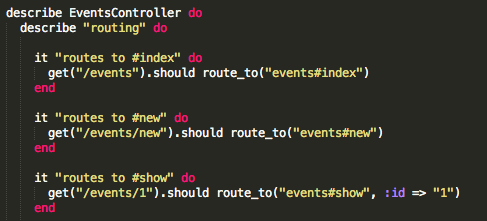
\includegraphics[scale=0.5]{images/project_management/testing/rspec_events_controller}
      \caption{Some of the Events Controller tests where readability is very clear due to RSpec}
      \end{figure}

      When a test fails the describe, context and it blocks are concatentated together into a very readable sentance which can be quickly understood by the user. 
      
      \begin{figure}[H]\centering
      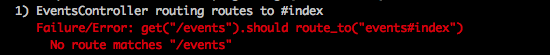
\includegraphics[scale=0.5]{images/project_management/testing/rspec_events_contoller_broken}
      \caption{Very readable broken test}
      \end{figure}

    \paragraph{factory\_girl:}
      `factory\_girl is a fixtures replacement with a straightforward definition syntax, support for multiple build strategies (saved instances, unsaved instances, attribute hashes, and stubbed objects), and support for multiple factories for the same class (user, admin\_user, and so on), including factory inheritance.'\cite{factory-girl}, it was particularly useful to us for creating valid models during testing that could then be modified in particular way to test a certain attribute/feature of a model.
      It also saved us from setting up the model multiple times during testing.
      It also became particularly relevant for seeing out database with test data to be displayed on the site, which made interacting with it during production far more realistic. Quite often seeding our database with a large amount of data allowed us to spot and address bugs that we may not have noticed otherwise.

    \paragraph{RSpec Guard:}
      `RSpec guard allows to automatically \& intelligently launch specs when files are modified'\cite{guard} and was incredibly useful to us when developing the back end code. To enable guard we type \verb!guard! and can leave it running in a terminal window. As the description states the tests are re run when a file is modified which allowed us immediatly to know if we'd broken the build before committing.
      Many times it saved us from committing broken code, and we even had it set up use OS X notifiers when the build was broken which meant we didn't even have to swap terminal screens to know if our code passed the tests.

      \begin{figure}[H]\centering
      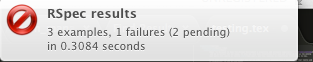
\includegraphics[scale=0.5]{images/project_management/testing/guard_osx}
      \caption{Mac OS X notification}
      \end{figure}

  \subsubsection{Client Side}
    \paragraph{Jasminerice:}
      For client side testing we chose to use Jasminerice since it is very similar to RSpec and thus does not require a vast amount of learning to get up to speed. Nicely guard also supports runing client side tests and thus the two could be merged together very easily without disrupting the development pattern.

  \subsubsection{Mocking}
    We made extensive use of mocking techniques when writing our test suite with the use of sinon.js\cite{sinon} and RSpec-mocks\cite{rspec_mocks}.

    We feel that mocking really helped us to to ensure that tests only failed when relevant code related to the class being tested was broken. Mock objects are used to test behaviour `much the same way that a car designer uses a crash test dummy to simulate the dynamic behavior of a human in vehicle impacts'\cite{mock_quote} and were of great importantance to us when testing a piece of code that depends on another.
    Since a specific test should only be testing a focus object, if an external object's behaviour was changed it and it broke a test it would have left us very confused to what functionality was actually broken. Mocking helped us avoid this problem, and some particular techniques for mocking we used were:
    
    \paragraph{Spies} enabled us to watch objects method calls. We could set an object up with a spy, run some code and then ensure that the spy was called, with the arguments we expected and called the expected number of times.

    \paragraph{Stubs} allowed us to decouple classes from one another during testing. We could stub out a classes new method in order to return our stubbed objects.
    These stubbed objects methods could be altered to return exactly what we wanted and they easily allowed us to test features of our code which would otherwise require a tricky set up.
    For example, when testing what happens when we fetch data from the server on the client side we could stub our model with the call to \verb!model.fetch([options])! yielding to either the success callback or the error callback.
    This nicely decoupled the server from our tests and easily allowed us to test error cases.



  \subsubsection{TDD}
    Due to time constraints and the majority of this project requring everybody learning new skills we adopted a slightly modified TDD approach. Since we'd decided it was best for people to become specialised in different areas Sarah read in depth about our chosen testing frameworks. After each stand up she speced out new unit tests for the next iteration which everyone else then wrote code to fix.